\documentclass[12pt,a4paper]{article}
%-- coding: UTF-8 --
\usepackage[UTF8]{ctex}
\usepackage[utf8]{inputenc}
\usepackage{geometry}
\usepackage{graphicx} % 引入图片
\usepackage{enumitem} % 取消列表默认间距
\geometry{left=3.18cm,right=3.18cm,top=2.54cm,bottom=2.54cm}
\usepackage{hyperref}
\hypersetup{hidelinks,
	colorlinks=true,
	allcolors=black,
	pdfstartview=Fit,
	breaklinks=true}
\usepackage{listings}
\usepackage{xcolor}
\usepackage{fontspec}
\usepackage{booktabs} % 三线表
\usepackage{float}

\usepackage{tikz}
\usepackage{amsmath}
\usepackage{colortbl}
\newcommand\y{\cellcolor{clight2}}
\definecolor{clight2}{RGB}{212, 237, 244}%
\newcommand\tikznode[3][]%
   {\tikz[remember picture,baseline=(#2.base)]
      \node[minimum size=0pt,inner sep=0pt,#1](#2){#3};%
   }
\tikzset{>=stealth}
\renewcommand\vec[1]{\mathbf{#1}}

% 嵌入代码风格
\lstset{
	language    = c++,
	breaklines  = true,
	captionpos  = b,
	tabsize     = 4,
	columns     = fullflexible,
	commentstyle = \color[RGB]{0,128,0},
	keywordstyle = \color[RGB]{0,0,255},
	basicstyle   = \small\ttfamily,
	stringstyle  = \color[RGB]{148,0,209}\ttfamily,
	rulesepcolor = \color{red!20!green!20!blue!20},
	showstringspaces = false,
}


%伪代码
\usepackage{multirow}
\usepackage{algorithm}
\usepackage[noend]{algpseudocode}
\usepackage{amsmath}

\title{实验四 \hspace{0.5cm} 动态规划}
\author{
\begin{tabular}{c @{\hspace{5mm}} c}
    黄韦杰 & 刘嘉杰 \\  % 作者名
    \href{mailto:hwj@hust.edu.cn}{hwj@hust.edu.cn} & \href{mailto:m202474039@hust.edu.cn}{m202474039@hust.edu.cn} % 邮箱
\end{tabular}
}
\date{October, 2024}

\begin{document}
\maketitle

\section{前言}
动态规划(dynamic programming)已经成为计算机科学中重要的算法设计范型。1957 年,Richard Bellman 在描述一类优化控制问题时创造了这个名字。那时,这个名字更多地用于描述问题,而不是解问题的技巧。规划(programming)意味着一系列的决策,而动态(dynamic)则传递着这样一种思想:所做决策可能依赖于当前状态,而与此前所做决策无关。此方法的主要特点是通过采用表格技术,用多项式算法代替指数算法。

动态规划典型的应用领域是组合优化问题,在这类问题中,可能有许多可行解(feasible
solution),每个解对应一个值,我们想要找出一个具有最优值的解,称这个解为问题的一个最优解,可能有多个解都能达到这个最优值。本质上,动态规划计算所有子问题的解,计算的过程从小问题到大问题,并将计算结果存储在一张表中,此方法的优点在于,一旦一个子问题被解决,就存储其结果,此后遇到同样的子问题,就不再重复计算。过去的五十多年,动态规划在运筹学、控制论、管理科学等领域的发展中,都发挥了无可比拟的领军作用,成为解决数学建模问题最常用的优化方法之一。但是,作为一个重要的最优化方法,它又存在着很多亟待解决的问题而显得很不完善。因此,在运用这个方法的过程中,人们一直致力于不断完善应用动态规划的条件以及动态规划问题的求解方法。诸如确定型一维动态规划的解析法、计算法等算法;确定型多维动态规划的拉格朗日乘子、逐次迭代、策略与函数空间近似、多项式逼近、超曲面搜索等算法;随机动态规划的基本算法等。

2018 年数学建模竞赛问题 B 智能 RGV的动态调度策略问题,该问题对动态规划方法有着深入的
应用,对参赛人员也提出了更高的要求,需要我们加以完善和优化。学习动态规划,这是一种解决棘手问题的方法,将问题分为小问题,并先着手解决这些小问题,聪明的你一定跃跃欲试,那还等什么,一起来感受动态规划的魅力吧!


\section{实验项目结构}

\begin{itemize}[noitemsep]
    \item[$-$] find\_maximum\_subarray \textit{题目一 \hspace{0.2cm}寻找最大子序列问题}
        \begin{itemize}[noitemsep]
            \item[$-$] include
                \begin{itemize}[noitemsep]
                    \item[$\bullet$] util.hpp \textit{常用函数头文件}
                    \item[$\bullet$] Solution.hpp \textit{待完成}
                \end{itemize}
            \item[$-$] data
            \item[$\bullet$] main.cpp \textit{主程序代码}
        \end{itemize}
    \item[$-$] longest\_common\_subsequence \textit{题目二 \hspace{0.2cm}最长公共子序列问题}
        \begin{itemize}[noitemsep]
            \item[$-$] include
                \begin{itemize}[noitemsep]
                    \item[$\bullet$] util.hpp \textit{常用函数头文件}
                    \item[$\bullet$] Solution.hpp \textit{待完成}
                \end{itemize}
            \item[$-$] data
            \item[$\bullet$] main.cpp \textit{主程序代码}
        \end{itemize}
\end{itemize}

\textcolor{red}{请注意,每次修改完代码之后,需要重新编译运行 main.cpp,如果直接执行上次编译好的 main.exe 或 main,新的修改将不会生效。在本地测试通过后请将
    代码提交到 OJ 上。}

\section{实验内容}

\subsection{寻找最大子序列问题}

给定一个长度为 $N$ 的数组 $A$,其任意连续子序列可以表示为 $A_i, A_{i+1}, \cdots, A_{j}$,其中 $0\le i \le j \le N-1$。最大子序列是指所有的子序列中和最大的那一个,注意子序列不能为空。为了降低难度,你只需要输出它的和,即:
$$result = \max_{0\le i\le j \le N-1}{\sum_{k=i}^j A[k]}$$

例如:[-2, 11, -4, 13, -5, -2] 的答案为 20。

请使用\textcolor{red}{动态规划}思想完成 Solution.hpp 的实现。

\begin{lstlisting}
    class Solution {
    public:
        long long find_maximum_subarray(vector<int> &A) {
            // 请在这里完成你的代码
        }
    };
\end{lstlisting}

测试数据范围:$N\le 10^6$, $|A[i]| \le 10^9$。



\subsection{最长公共子序列问题}

给定两个字符串 $s, t$,求出它们的最长公共子序列长度。

\begin{lstlisting}
    class Solution {
        // 用于调试输出二维数组
        void print_table(vector<vector<int>> &table) {
            debug(table);
        }
    public:
        int lcs(string s, string t, vector<vector<int>> &c,
                vector<vector<int>> &b) {
            // 注意,string 类型是 C++ 的字符串类型,可以通过 s[0] 来访问 s 的第一个字符
            int n = s.size(), m = t.size();
            c.resize(n + 1);
            b.resize(n + 1);
            for(int i = 0; i <= n; i++) {
              c[i].resize(m + 1, 0);
              b[i].resize(m + 1, 0);
            }
            // 以上是数组初始化操作,请在下面完成你的代码
        }
    
        // print_lcs 只用于自己调试输出最长公共子序列,不做正确性检测
        void print_lcs(vector<vector<int>> &b, string &s, int i, int j) {
            // 请在这里完成你的代码
        }
    };
\end{lstlisting}

main.cpp 的 main 函数中配置了简单的样例测试,你可以在写代码时首先观察这一组数据能否输出正确结果。调试成功后,\textcolor{red}{再取消掉最后 test() 的注释进行所有测试数据的运行检测。另外,你可以选择性的实现\textbf{print\_lcs}函数,来帮助你调试代码,该函数不影响最终结果}

\begin{lstlisting}
    int main(){
        string s = "AGCTAG";
        string t = "ACTCC";
        int n = s.size(), m = t.size();
        vector<vector<int>> b, c;
    
        Solution sol;
        // 求解 LCS 长度
        int res = sol.lcs(s, t, c, b);
        cout << BLUE << "[test case]" << END << endl;
        cout << "s: " << s << endl;
        cout << "t: " << t << endl;
        cout << "Length of LCS: " <<  res << endl;
        cout << "LCS is: ";
        sol.print_lcs(b, s, n, m);
        cout << endl;
    
        // test();
    
        return 0;
    }
\end{lstlisting}




\section{实验思考}

\begin{enumerate}
    \item 在寻找最大子序列问题中,对比分治算法与动态规划算法在时空复杂度上的不同。
    \item 分析动态规划方法求解最长公共子序列问题的时空复杂度。
    \item 请解释最长公共子序列问题中,$c[i][j]$ 的 $i$ 和 $j$ 分别是什么含义,$c[i][j]$ 的值又是什么含义。
    \item 你认为使用动态规划解决问题的难点是什么?除课堂所讲内容外,有哪些比较典型的动态规划类型?
\end{enumerate}

\section{拓展实验(仅供参考,实际以OJ上为准)}

给定一个仅包含 0 和 1 、大小为 $rows \times cols$ 的二维二进制矩阵,找出只包含 1 的最大矩形,并返回其面积。

例如下图所示的 01 矩阵,最大全 1 子矩阵面积为 6:

\begin{figure}[h]
    \centering
    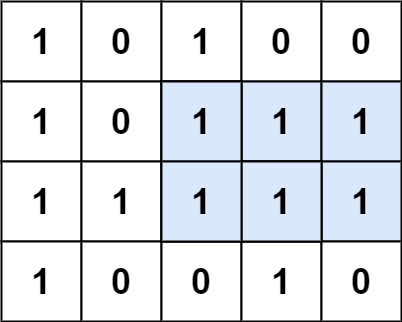
\includegraphics[width=4cm]{img/lab4/maximal.jpg}
\end{figure}

数据范围:$1\le row, cols \le 200$

你可以在这里完成本拓展题目:\href{https://leetcode.cn/problems/maximal-rectangle/}{https://leetcode.cn/problems/maximal-rectangle/}

\textbf{提示:} 为了通过本题测试,你需要使用不超过 $O(n^3)$ 时间复杂度的算法。可以尝试枚举子矩阵的上边界与下边界,然后将问题转换为你熟悉的题目。

\section*{更新历史}

\begin{center}
    \begin{tabular}{|c|c|c|}
        \hline
        \textbf{更新时间} & \textbf{助教} & \textbf{更新内容} \\
        \hline
        2024 & 黄韦杰, 刘嘉杰 & 完善前言与实验思考,修正数据范围\\
        2023 & 王梓健, 黄韦杰 & 添加 OJ 相关表述,完善本地环境使用方法 \\
        2022 & 邢广杰, 李晓晓 & 完善实验题目,开始更新记录 \\
        2021 & 韩耀东 & 主要内容构建 \\
        % Add more rows as needed
        \hline
        \end{tabular}
\end{center}

\end{document}